% CVPR 2026 Paper Template; see https://github.com/cvpr-org/author-kit

\documentclass[10pt,twocolumn,letterpaper]{article}

%%%%%%%%% PAPER TYPE  - PLEASE UPDATE FOR FINAL VERSION
\usepackage{cvpr}              % To produce the CAMERA-READY version
% \usepackage[review]{cvpr}      % To produce the REVIEW version
% \usepackage[pagenumbers]{cvpr} % To force page numbers, e.g. for an arXiv version

\usepackage{float}

% Import additional packages in the preamble file, before hyperref
\input{preamble}

% It is strongly recommended to use hyperref, especially for the review version.
% hyperref with option pagebackref eases the reviewers' job.
% Please disable hyperref *only* if you encounter grave issues,
% e.g. with the file validation for the camera-ready version.
%
% If you comment hyperref and then uncomment it, you should delete *.aux before re-running LaTeX.
% (Or just hit 'q' on the first LaTeX run, let it finish, and you should be clear).
\definecolor{cvprblue}{rgb}{0.21,0.49,0.74}
\usepackage[pagebackref,breaklinks,colorlinks,allcolors=cvprblue]{hyperref}


%%%%%%%%% TITLE - PLEASE UPDATE
\title{Course Project 1: Linear SVM on AwA2 Deep Features}

%%%%%%%%% AUTHORS - PLEASE UPDATE
\author{Zhiyang Tang\\523031910097}

\begin{document}
\maketitle
\section{Experimental Setting}
We use the provided AwA2 deep feature benchmark for Question 1 and Question 2. The dataset contains 37,322 images from 50 animal categories. Following the project requirement, each category is split independently into 60\% training samples and 40\% testing samples, which produces 22,373 training instances and 14,949 testing instances in total. The input representation is the released 2048-dimensional ResNet101 feature for each image, so the classifier is trained directly on high-level semantic features rather than raw pixels.

For classification, we adopt a linear Support Vector Machine implemented by \texttt{LinearSVC}. To select a suitable regularization strength, we run 5-fold stratified cross-validation on the training split and search over $C\in\{0.01,0.1,1,10,100\}$. The best hyper-parameter selected by cross-validation is $C=0.01$. All experiments use a fixed random seed of 42 for reproducibility. The entire training and evaluation pipeline takes about 56.95 minutes on the current machine.

\begin{figure}[H]
    \centering
    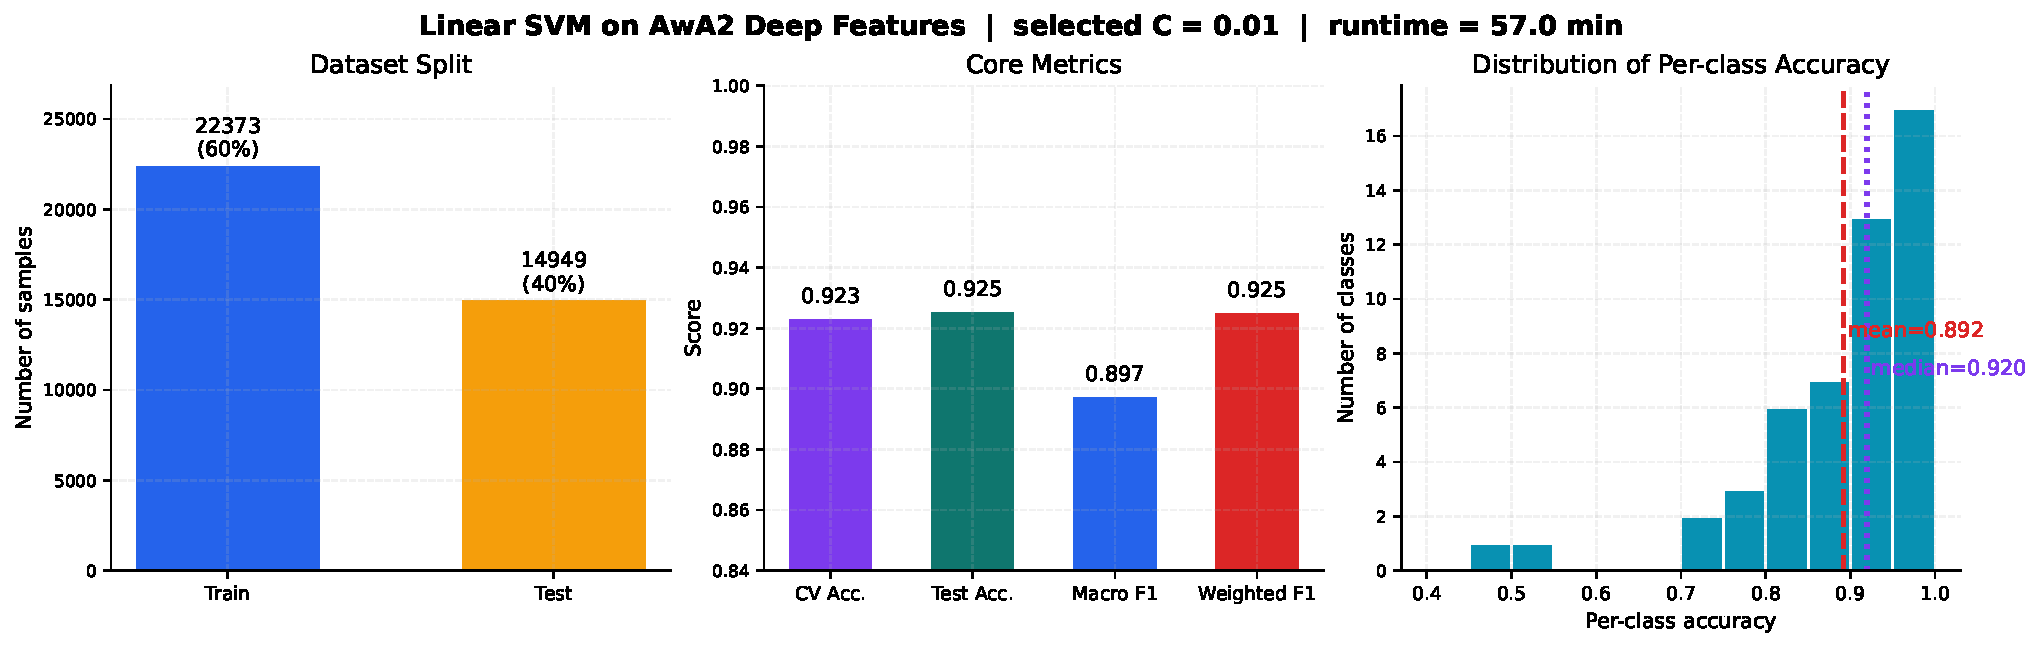
\includegraphics[width=\linewidth]{figures/q1_q2_overview.pdf}
    \caption{Overall experimental summary. Left: class-wise 60/40 train-test split. Middle: cross-validation accuracy, final test accuracy, macro F1 and weighted F1. Right: distribution of per-class test accuracy.}
    \label{fig:overview}
\end{figure}

\section{Experimental Results}
The final linear SVM achieves a test accuracy of \textbf{92.52\%}, which is slightly higher than the best cross-validation accuracy of \textbf{92.30\%}. In addition, the macro F1 score is \textbf{89.70\%} and the weighted F1 score is \textbf{92.47\%}. This gap between macro and weighted F1 indicates that the classifier is very strong overall, but its performance is not perfectly uniform across all categories. The histogram in Figure~\ref{fig:overview} confirms this observation: the median per-class accuracy is about 0.920, while the mean per-class accuracy is about 0.892 because a small number of difficult categories pull the average down.

\begin{figure*}[t]
    \centering
    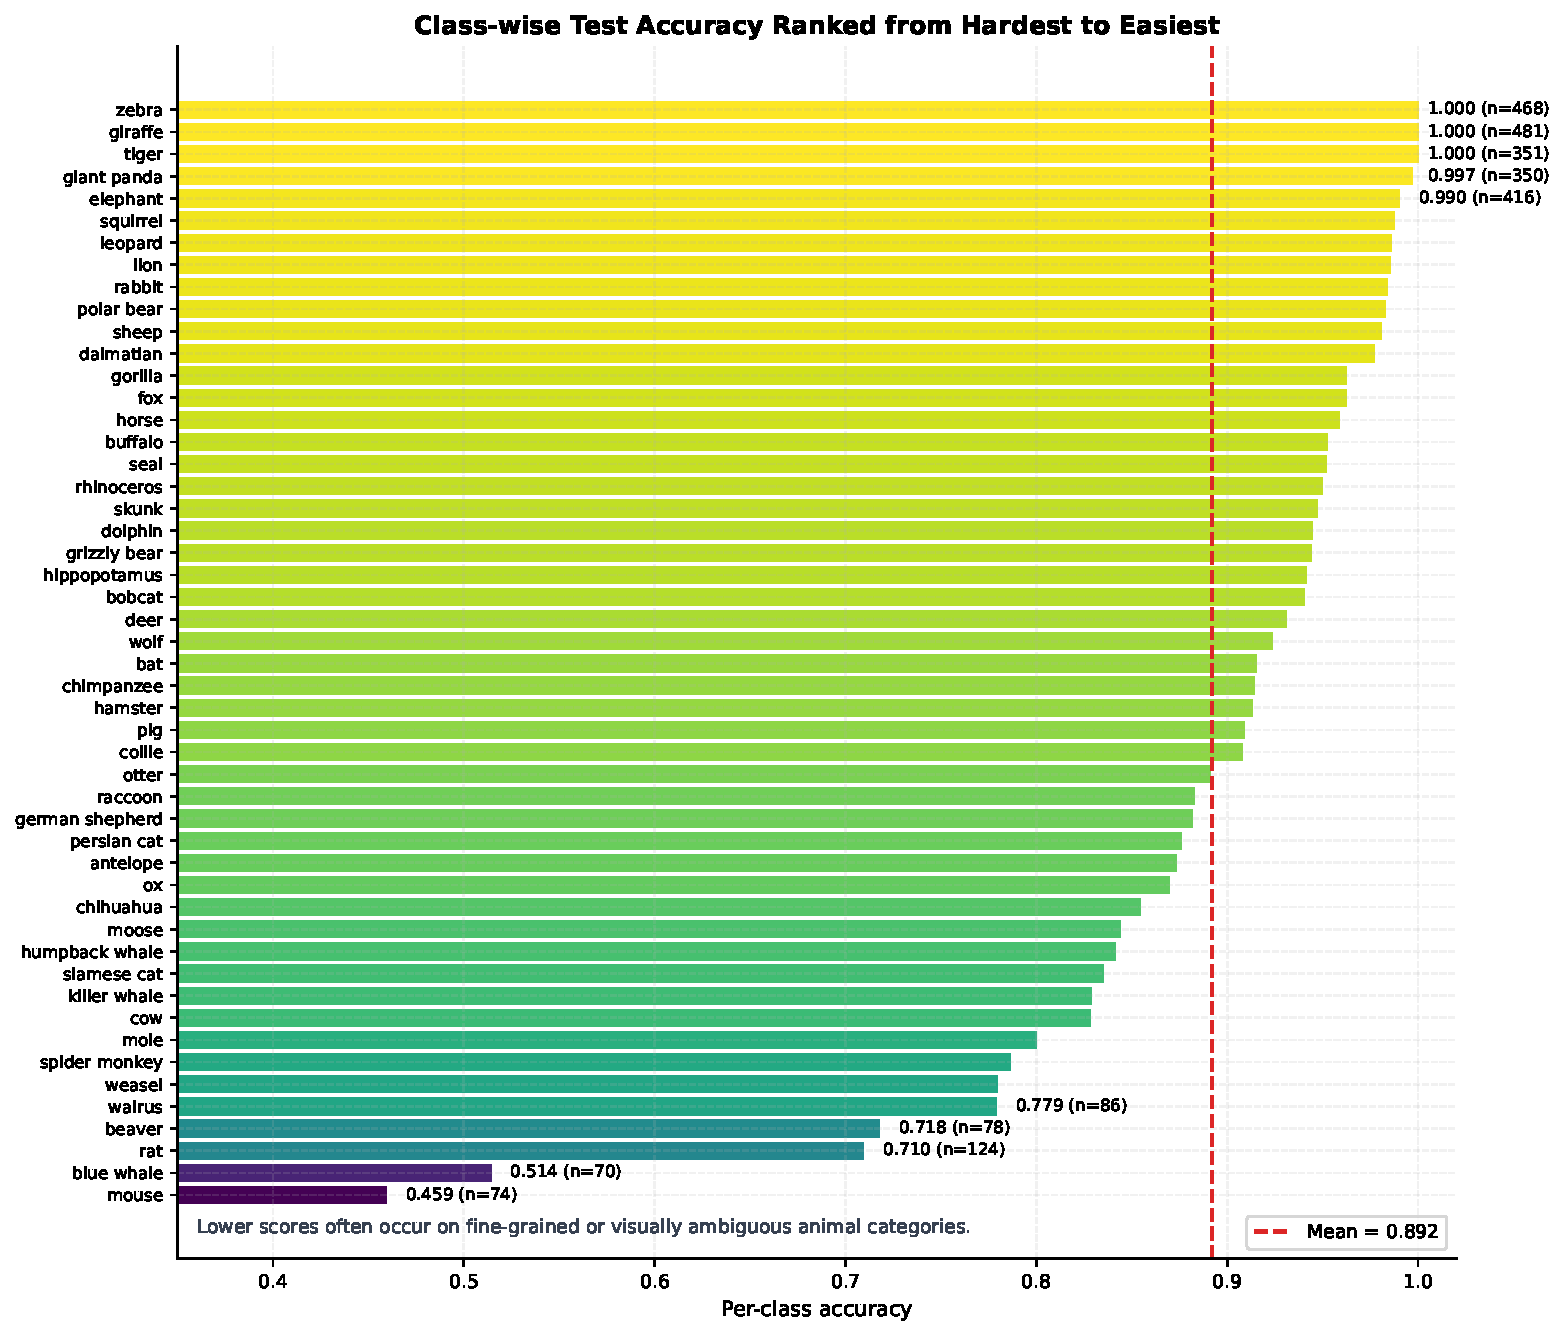
\includegraphics[width=0.56\linewidth]{figures/q1_q2_ranked_accuracy.pdf}\hfill
    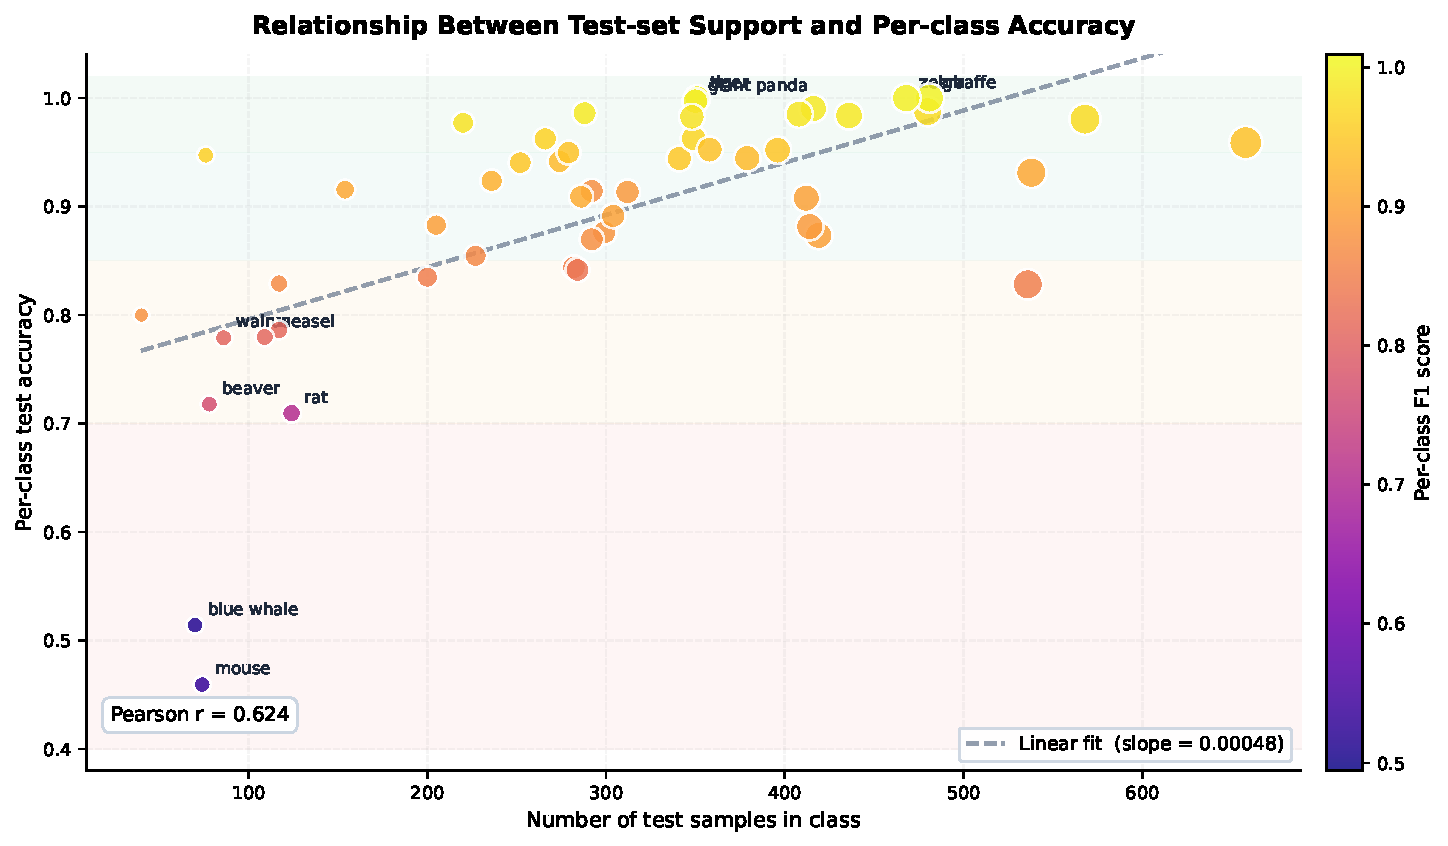
\includegraphics[width=0.41\linewidth]{figures/q1_q2_support_vs_accuracy.pdf}
    \caption{Detailed class-wise analysis. Left: per-class test accuracy ranked from the most difficult class to the easiest class. Right: relationship between test-set support and class accuracy, where color encodes per-class F1 score.}
    \label{fig:class_analysis}
\end{figure*}

Figure~\ref{fig:class_analysis} provides a more detailed interpretation. First, the ranking plot shows that a large portion of categories are recognized very reliably: 30 out of 50 classes achieve at least 90\% accuracy, and 17 classes reach at least 95\% accuracy. Some classes are classified almost perfectly, including \textit{tiger}, \textit{giraffe}, and \textit{zebra}, each with 100\% accuracy, together with \textit{giant panda} (99.71\%), \textit{elephant} (99.04\%), and \textit{lion} (98.53\%). These results suggest that the deep features already separate visually distinctive large mammals extremely well, so a linear decision boundary is sufficient.

Second, the weakest categories are concentrated in a small set of visually ambiguous animals. The most difficult class is \textit{mouse} with 45.95\% accuracy, followed by \textit{blue whale} (51.43\%), \textit{rat} (70.97\%), \textit{beaver} (71.79\%), \textit{walrus} (77.91\%), \textit{weasel} (77.98\%), and \textit{spider monkey} (78.63\%). These lower scores are reasonable because such categories either have limited samples, large appearance variation, or strong similarity to other animals. Therefore, the main error source is not the inability of the model to fit the training data globally, but the residual confusion among a few hard semantic classes.

Third, the scatter plot reveals a positive relationship between the number of test samples and the per-class accuracy, with Pearson correlation about \textbf{0.624}. In other words, categories with more examples generally obtain more stable and higher scores, while categories with fewer samples are more vulnerable to under-representation and intra-class variation. This trend explains why macro F1 is lower than weighted F1: underperforming classes tend to be relatively small, so they hurt the unweighted class average more than the overall sample-weighted metric.

Overall, the results show that deep features extracted by ResNet101 are already highly discriminative for AwA2, and a simple linear SVM can exploit them effectively. The remaining room for improvement is concentrated on low-support and visually confusing classes rather than on the dataset as a whole.

\section{Conclusion}
This experiment verifies that a linear SVM is a strong and efficient classifier on top of pretrained deep features. With only a linear decision function and a small hyper-parameter search, the model reaches 92.52\% test accuracy on the AwA2 benchmark. The analysis also shows that performance differences mainly come from a handful of difficult categories, especially those with fewer samples or stronger visual overlap. A natural next step would be feature normalization, hard-class analysis through a confusion matrix, or trying a non-linear classifier to further improve the tail classes.

\end{document}
